
\documentclass{article}
\usepackage{amsmath}
\usepackage{graphicx}
\DeclareMathOperator{\Div}{div}
\DeclareMathOperator{\Rot}{rot}
\newcommand{\parder}[2]{\frac{\partial {#1}}{\partial {#2}}}

\author{Julien Carayol}
\title{Fiche de SC411}
\begin{document}
%\maketitle
\newpage
\section{Électromagnétisme}
\subsection{Équations de Maxwell}

  \[\vec{\nabla}.\vec{D}=\Div\vec{D}=\rho\]
  \[\vec{\nabla}.\vec{B}=\Div\vec{B}=0\]
  \[\vec{\nabla}\wedge\vec{E}=\Rot\vec{E}=-\parder{\vec{B}}{t}\]
\[\vec{\nabla}\wedge\vec{H}=\Rot\vec{H}=\parder{\vec{E}}{t} +\vec{J} \]
\\Avec
\[\vec{D}=\varepsilon\vec{E}\;\;\;\;\;\;\;\;\;\;\vec{B}=\mu\vec{H}\]
\\Et \[c^2=\frac{1}{\varepsilon_0\mu_0}\]
\section{Lignes de transmission}
\[\left( \begin{array}{c}
a\\
b\\
c
\end{array} \right)\]
\subsection{Paramètres linéiques}
\begin{center}
  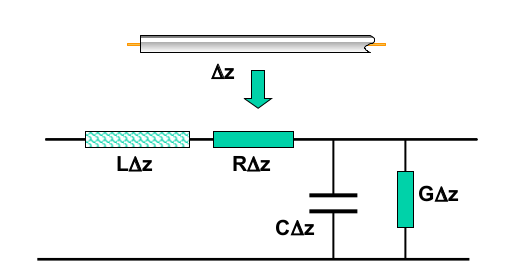
\includegraphics[scale=0.5]{/home/julien/lateX/src/Paramlineiques.png}
\end{center}
\end{document}
\begin{array}{c}
a\\
b\\
c
\end{array}
